\documentclass[micros_g1_main.tex]{subfiles}
\begin{document}

\section{}

Se midi\'o el tiempo de acceso de la memoria flash: desde que se activa chip enable (en este caso desde que pasa de 1 a 0, pues es active low), hasta que se tiene el dato le\'ido en el bus. 

Para determinar cu\'ando ocurre esto, se tuvo en cuenta que el bus de datos se multiplexa con el LSB de la direcci\'on. Se busc\'o una posici\'on de memoria de la flash que fuera par y tuviese guardado un dato impar, o viceversa. De esta manera, el bit menos significativo conmuta cuando se lee el dato. Se encontr\'o que en la posici\'on C001, el dato era 10, lo cual cumple este requisito. Alterando el programa del ejercicio 1 para que se accediera a esta posici\'on en lugar de a la C000, se realiz\'o la medici\'on que se observa en la figura \ref{fig:t-acceso}.

\begin{figure}[ht]
	\centering
	\fbox{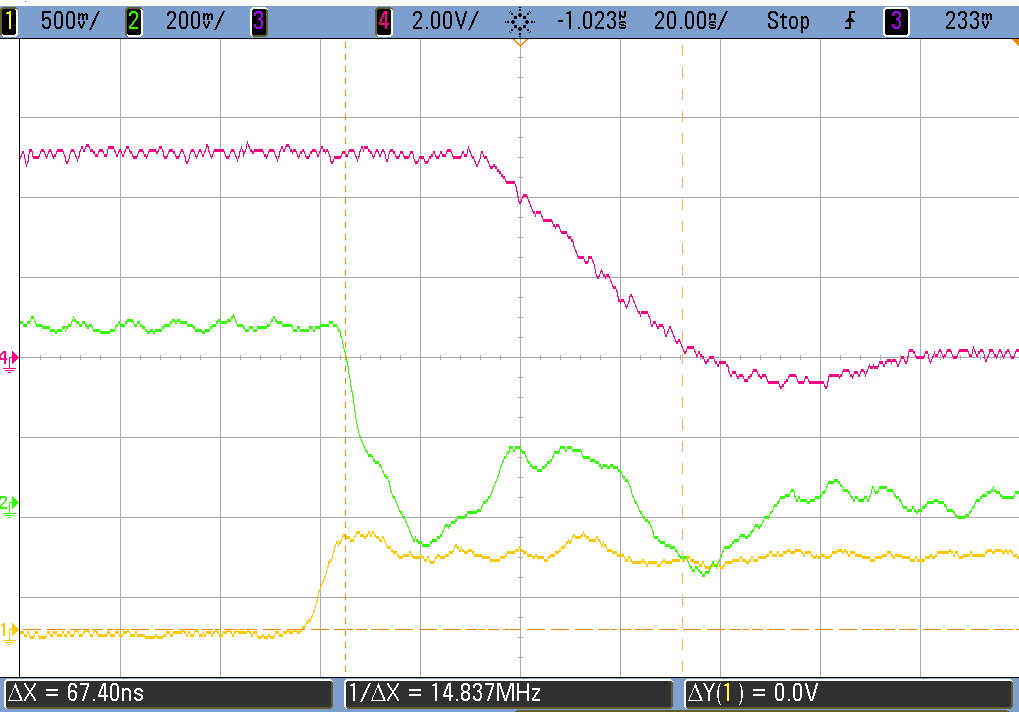
\includegraphics[width=\textwidth]{images/micros-g1-ej3.png}}
	\caption{Medici\'on del tiempo de acceso de la memoria flash. Se\~nales representadas: E (amarillo), $\overline{\text{CE}}$ (verde), D0 (rosa)}
	\label{fig:t-acceso}
\end{figure}

Se observa que el tiempo de acceso es de alrededor 67ns. En la primera parte de este tiempo, aproximadamente 20ns, no se observan cambios en la se\~nal D0, lo cual suger\'ia que este es el tiempo de propagaci\'on de la se\~nal de chip enable en la memoria. Los restantes $\sim$50ns corresponden al tiempo que tarda al bus de datos en cambiar de estado.

\end{document}
